\documentclass[twocolumn]{article}
\usepackage[utf8]{inputenc}
\usepackage[landscape, total={10in,8in}]{geometry}
\setlength{\columnsep}{.5in}
\usepackage{graphicx}
\graphicspath{{./}}
\usepackage[font=Large,labelfont=bf]{caption}
\captionsetup{width=\linewidth}

\begin{document}

	\begin{figure}
			\centering 
			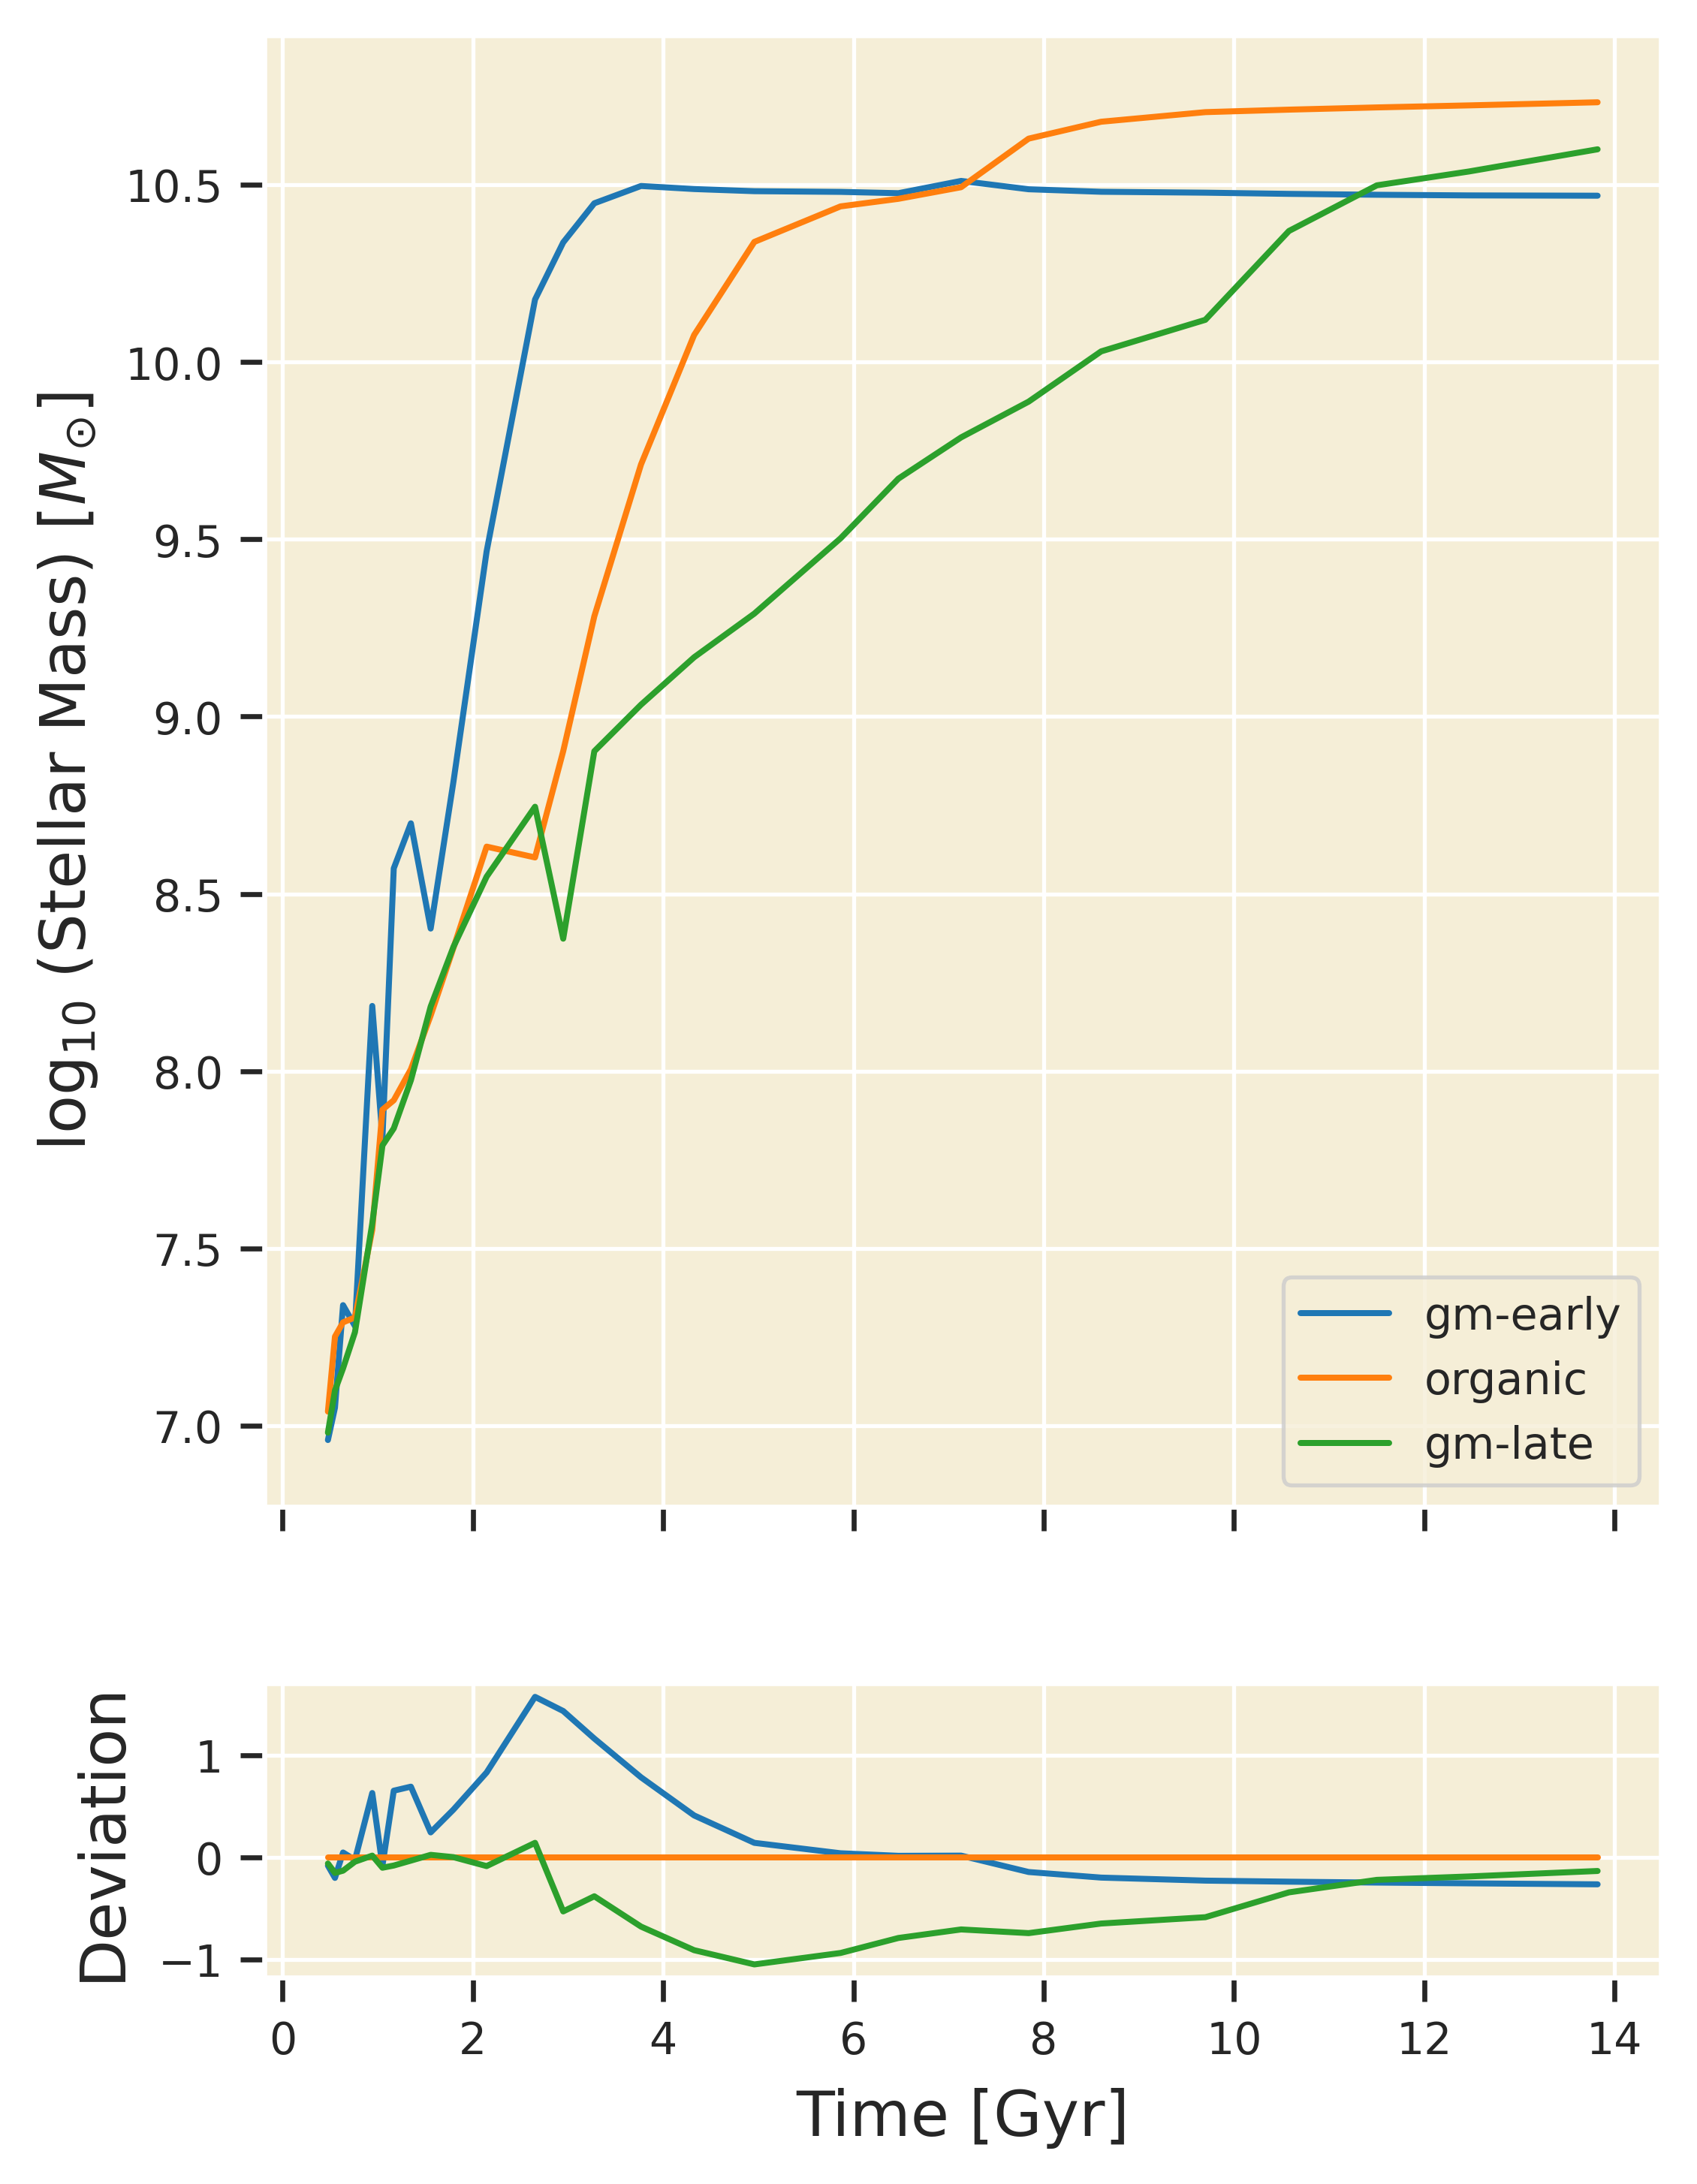
\includegraphics[width=\columnwidth]{./Stellar_mass.png}
			\caption{Stellar mass variation.}
	\end{figure}

	\begin{figure}
			\centering 
			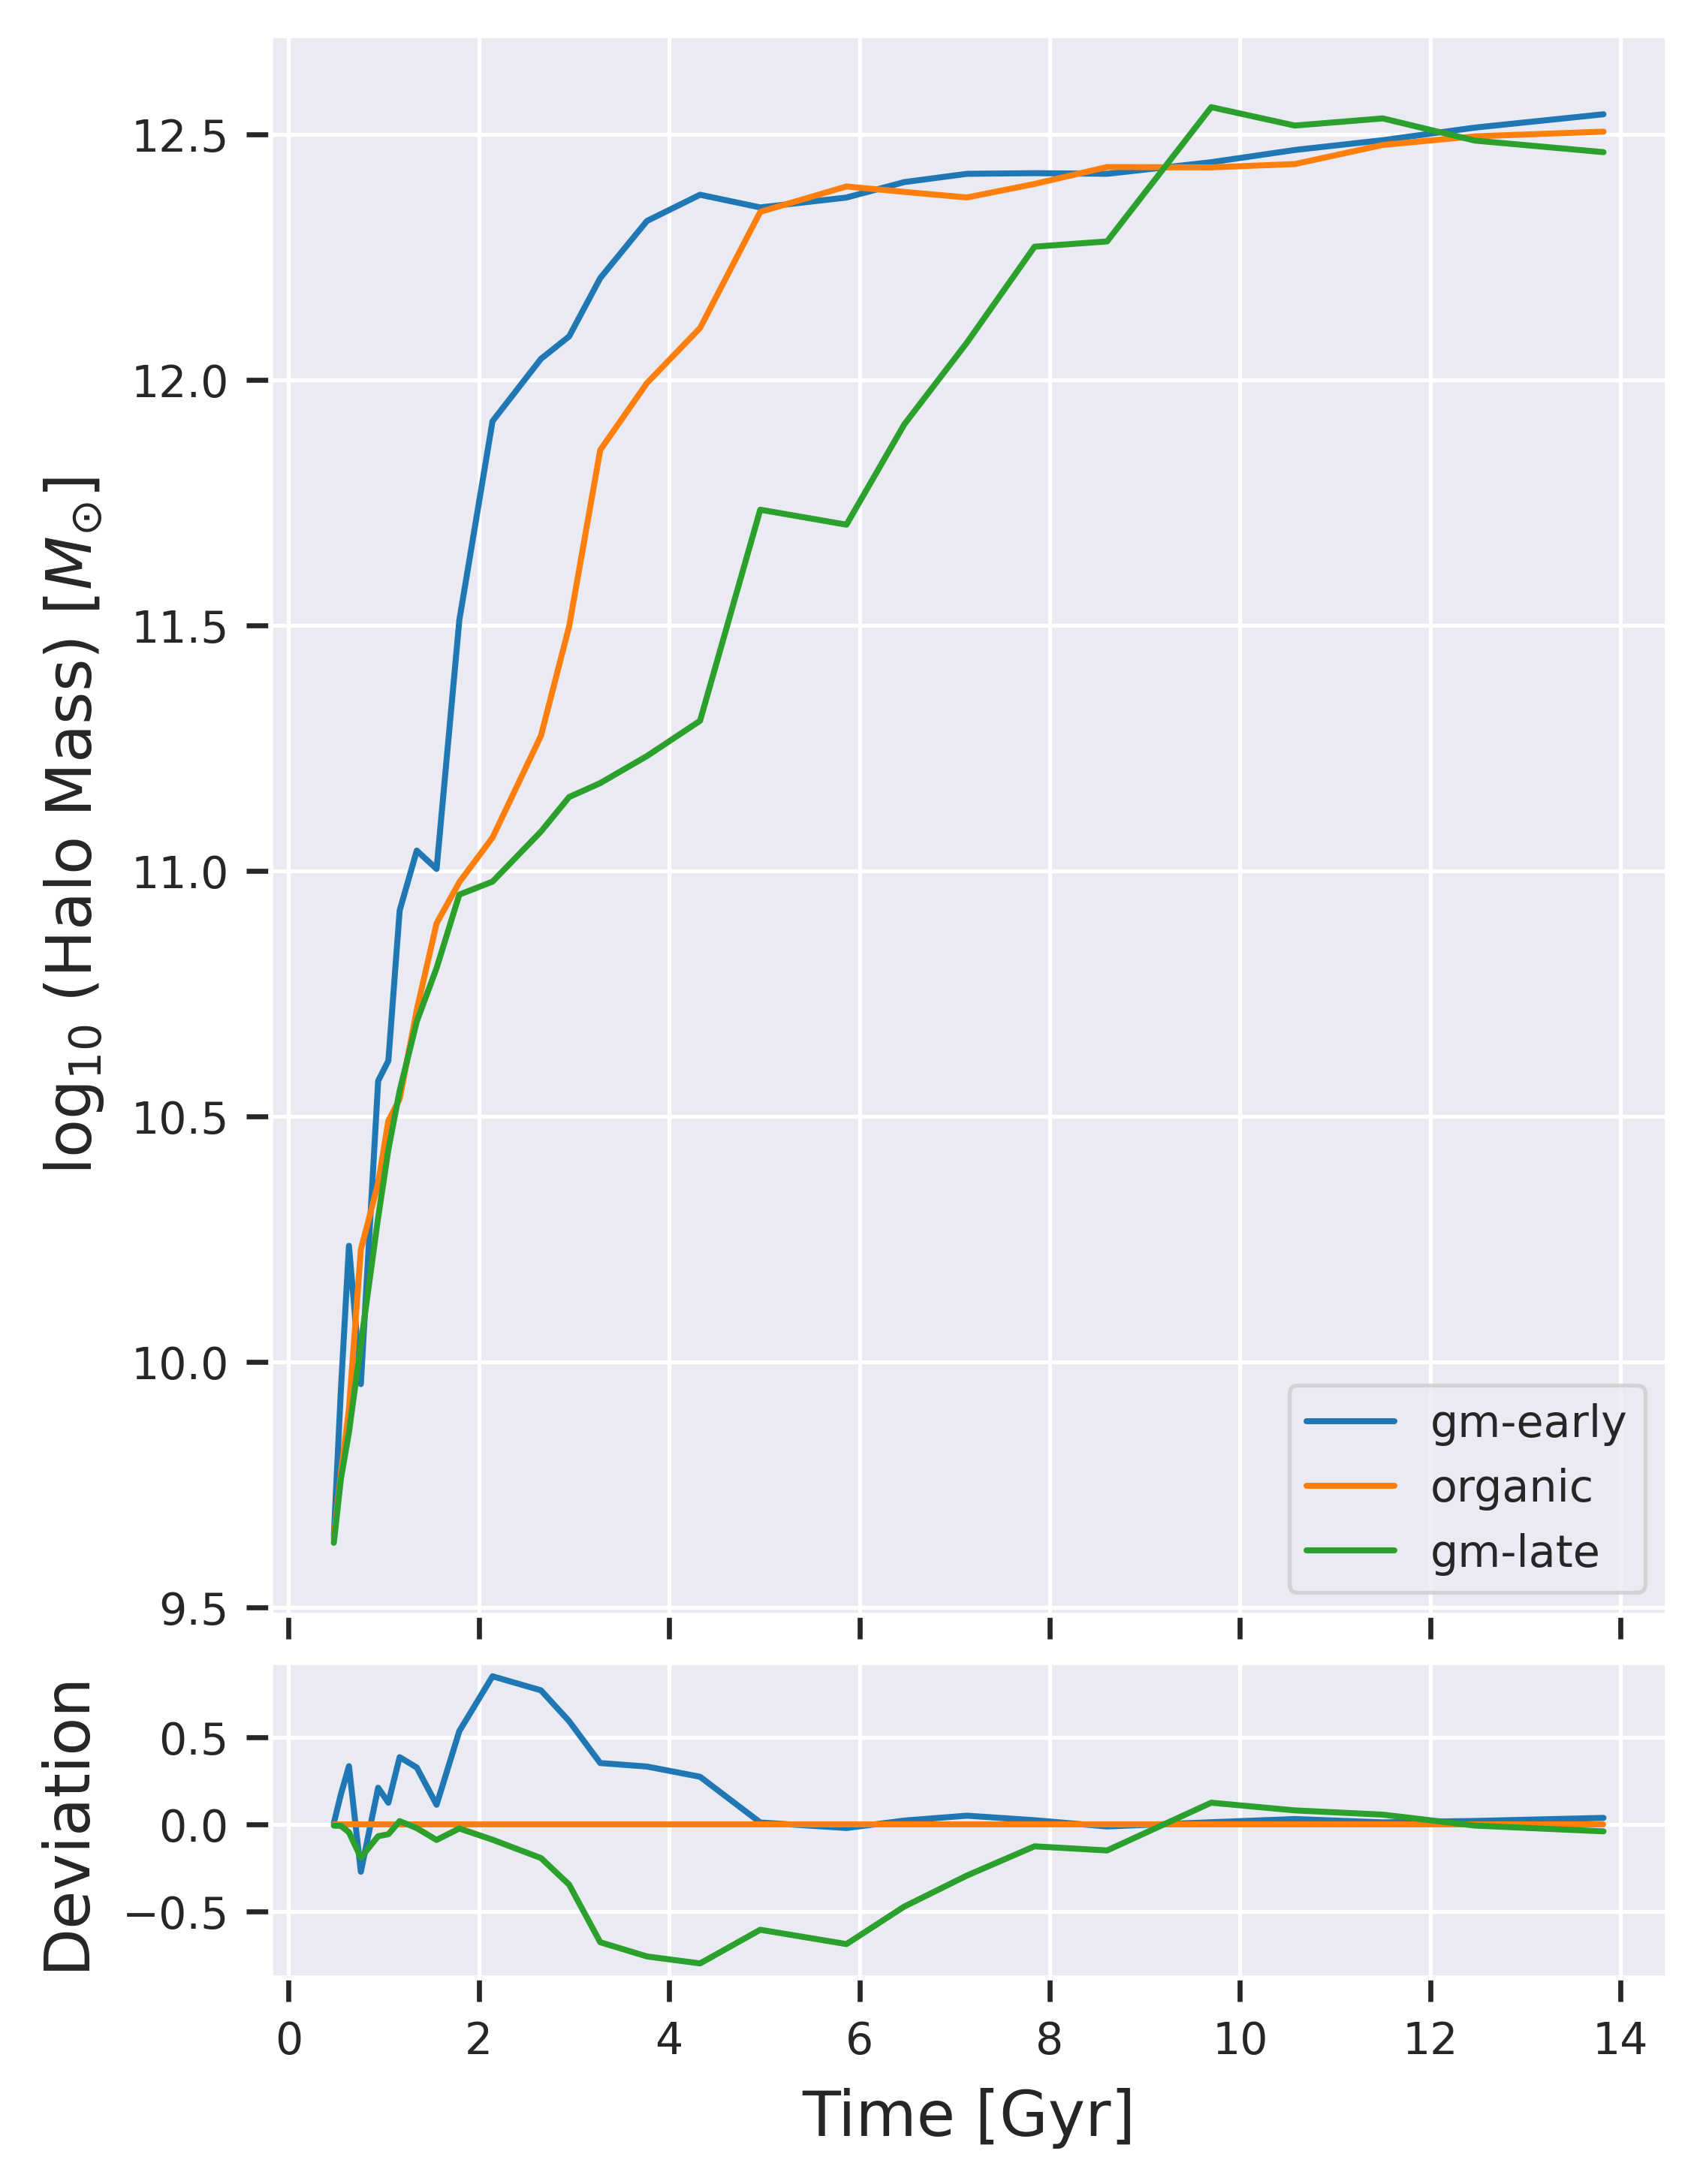
\includegraphics[width=\columnwidth]{./Halo_mass.png}
			\caption{Halo mass variation.}
	\end{figure}
	
	\begin{figure}
			\centering 
			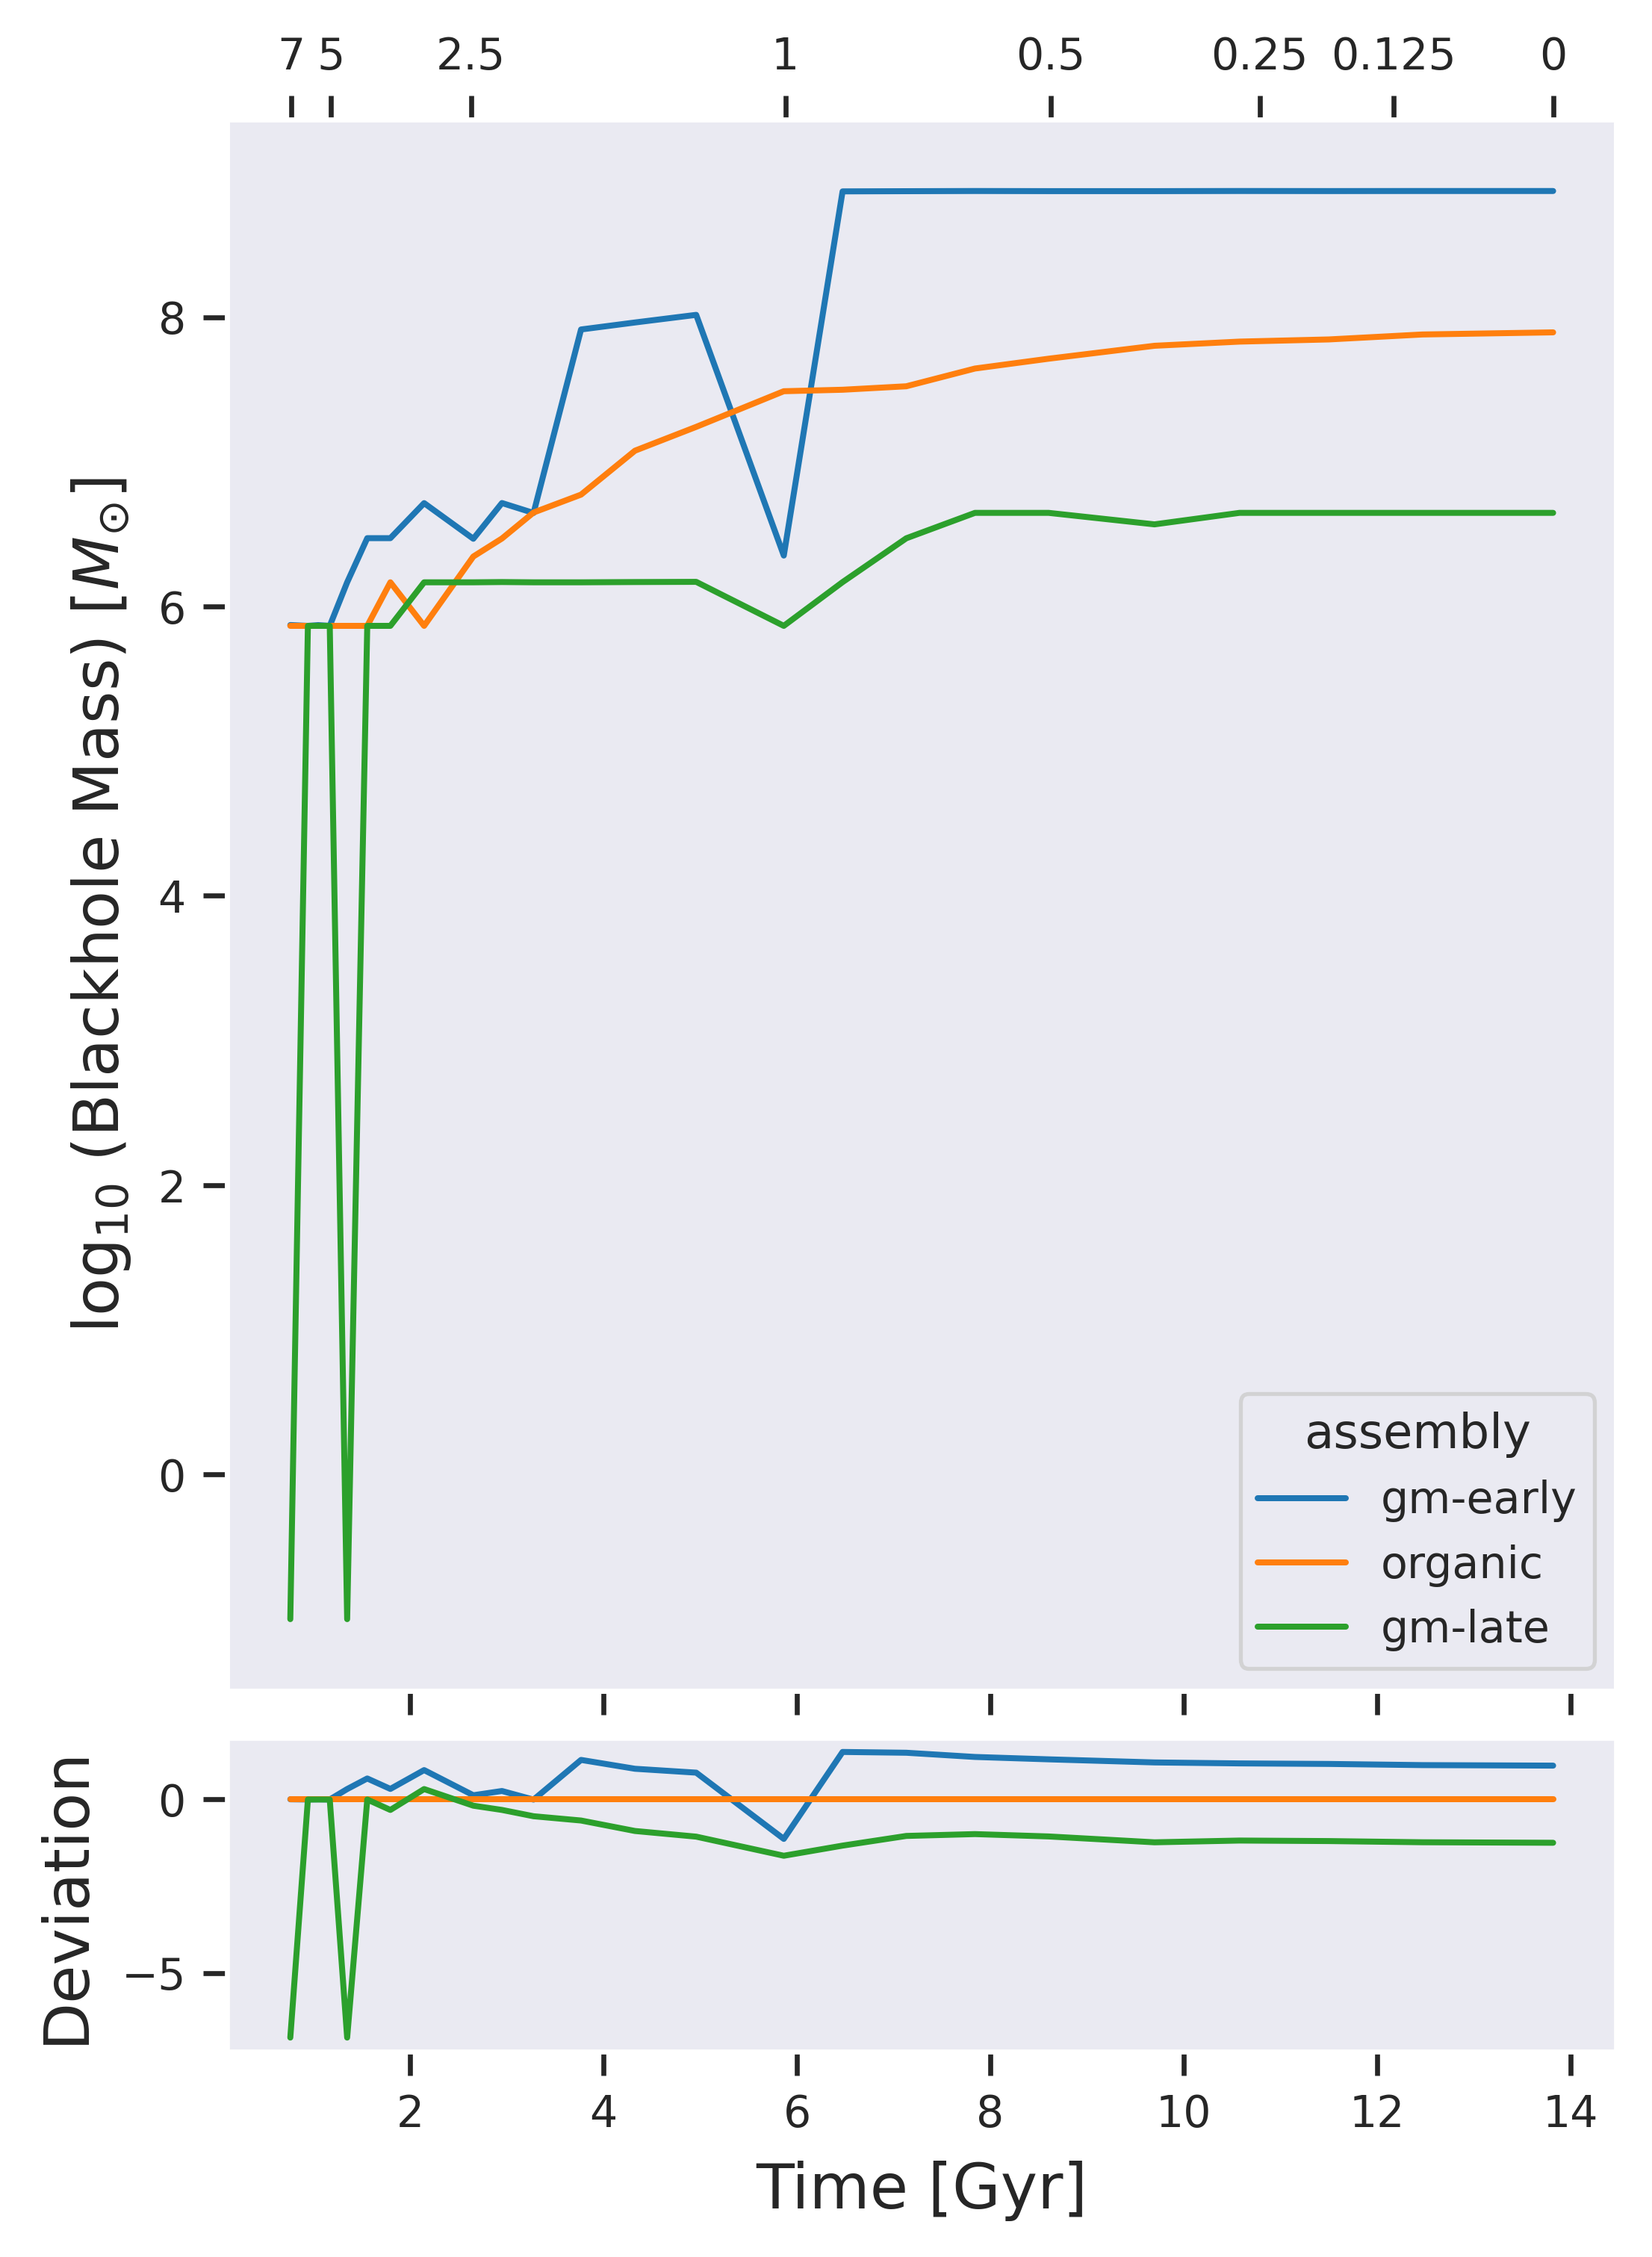
\includegraphics[width=\columnwidth]{./BH_mass.png}
			\caption{Blackhole mass variation.}
	\end{figure}

	\begin{figure}
			\centering 
			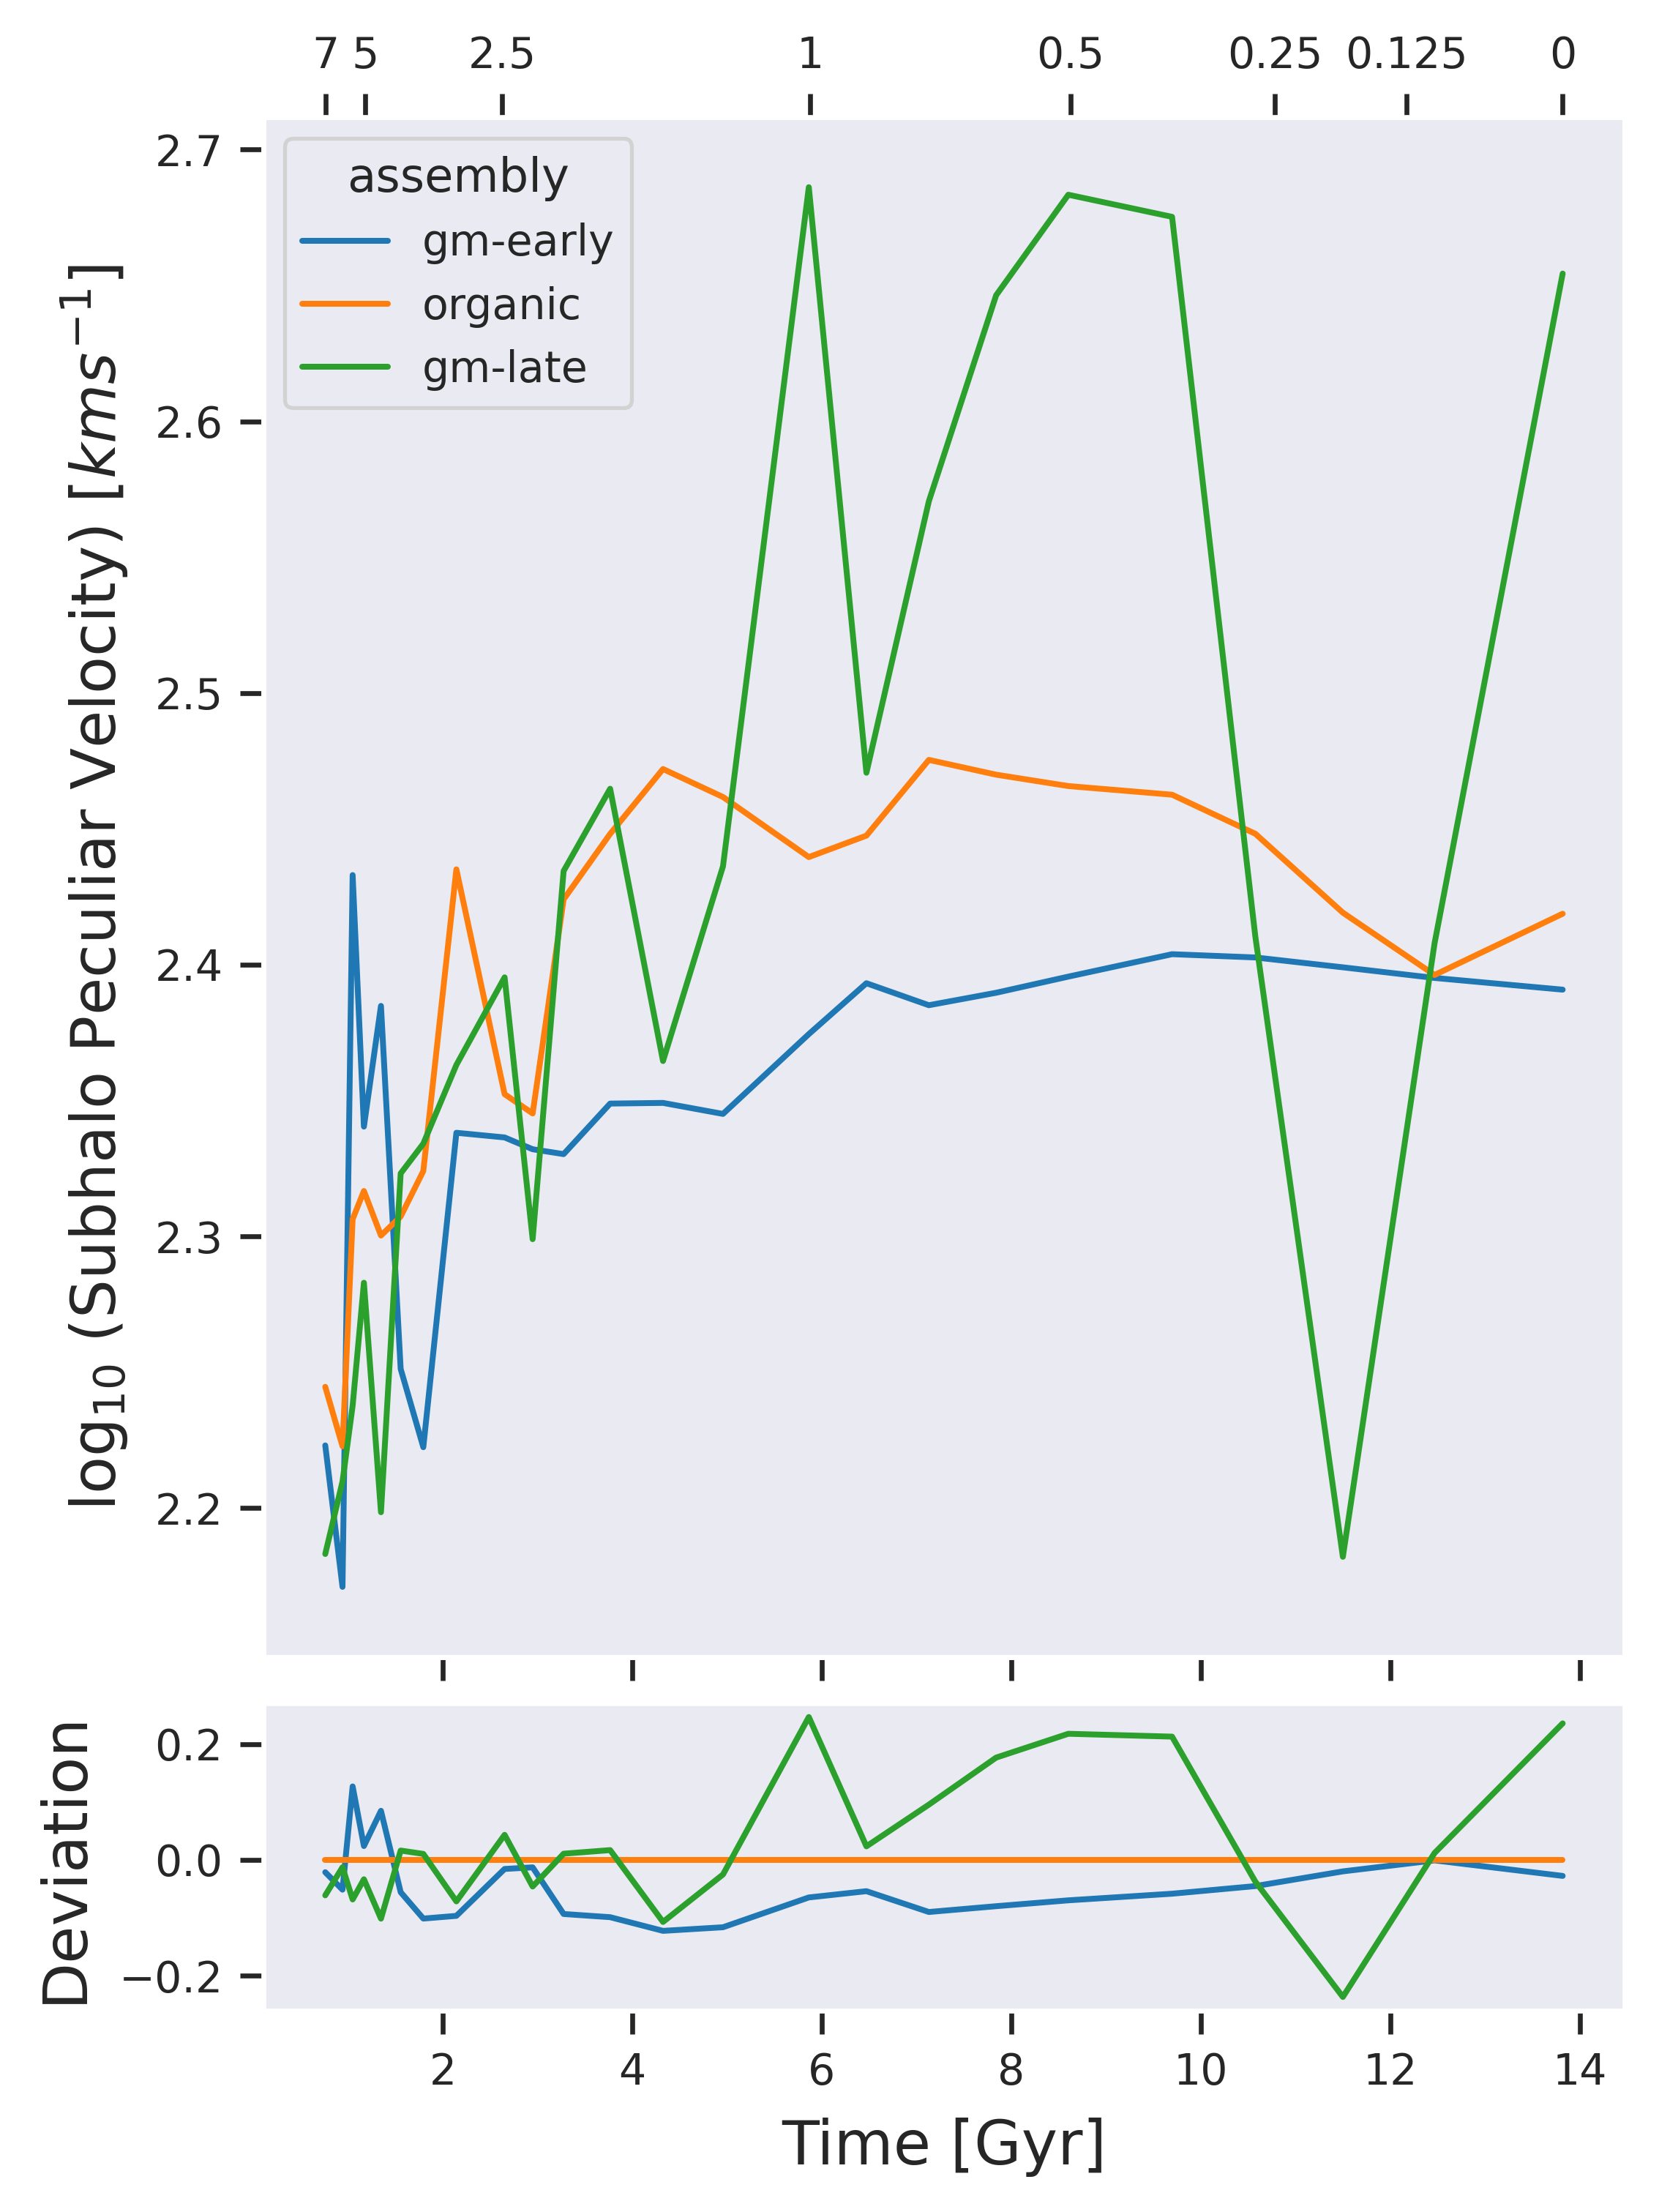
\includegraphics[width=\columnwidth]{./subhalo_peculiar_velocity.png}
			\caption{Subhalo peculiar velocity (Euclid norm) variation.}
	\end{figure}

	\begin{figure}
			\centering 
			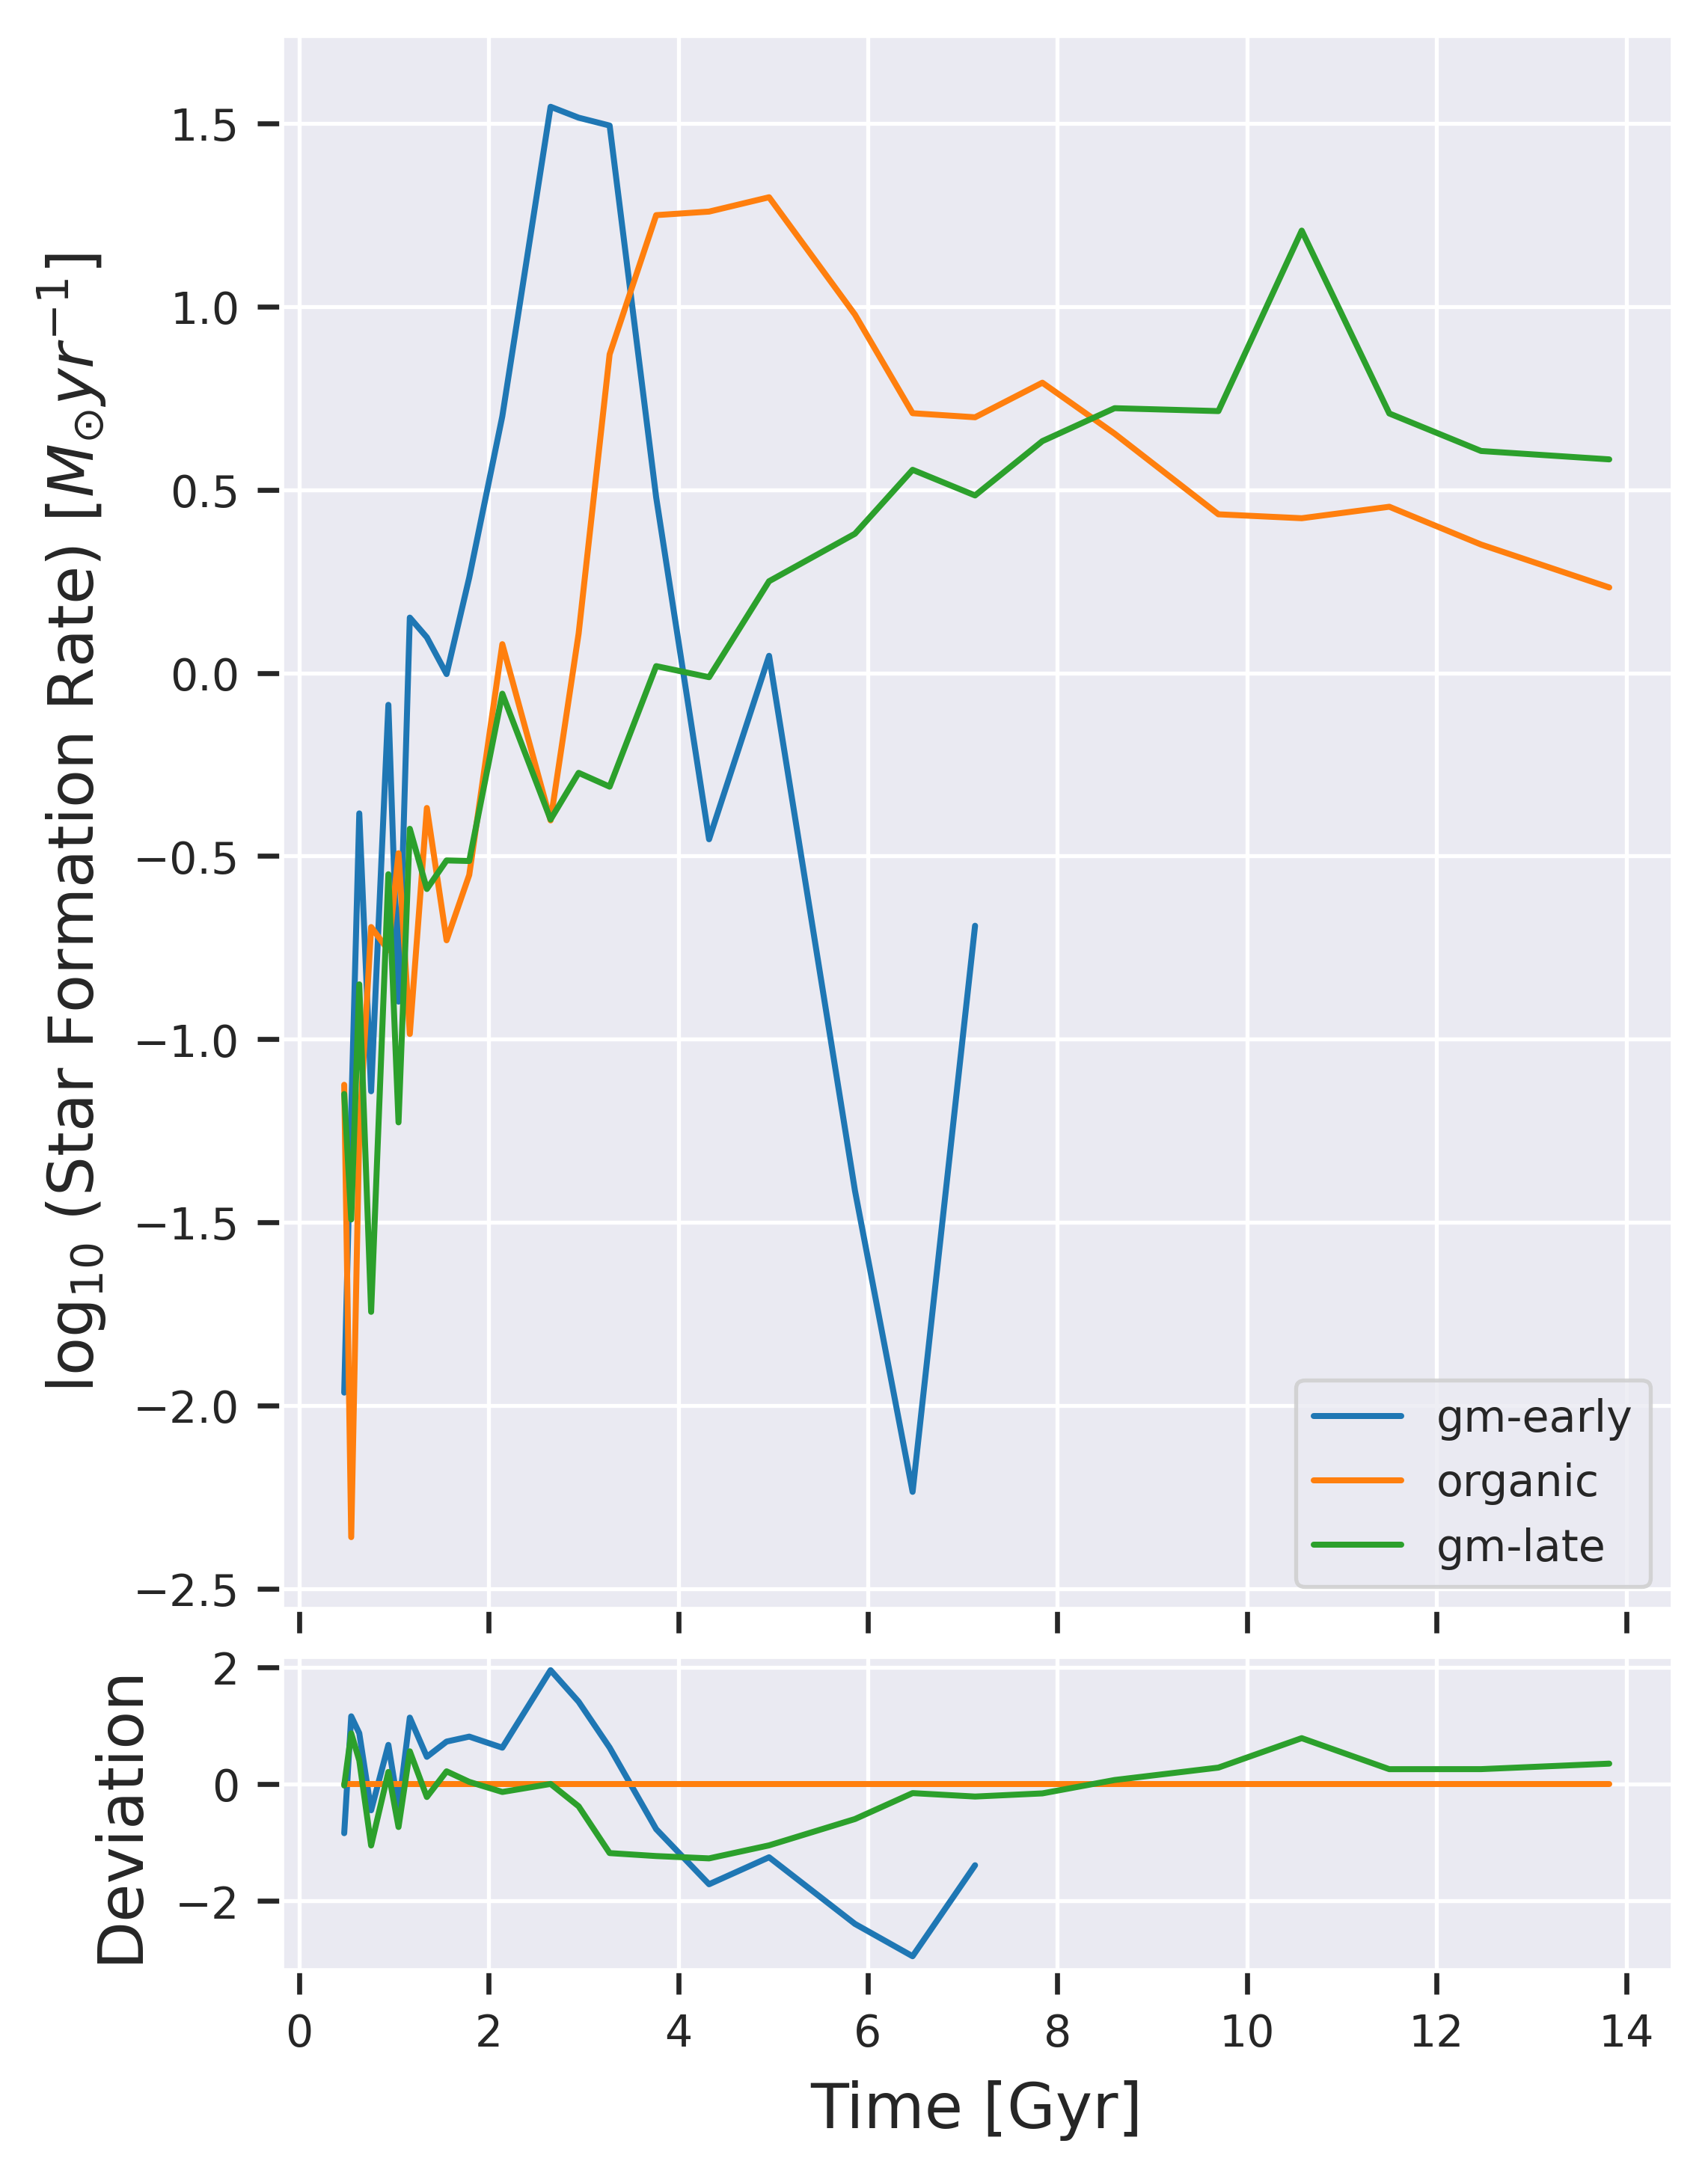
\includegraphics[width=\columnwidth]{./SFR.png}
			\caption{Star formation rate variation.}
	\end{figure}

	\begin{figure}
			\centering 
			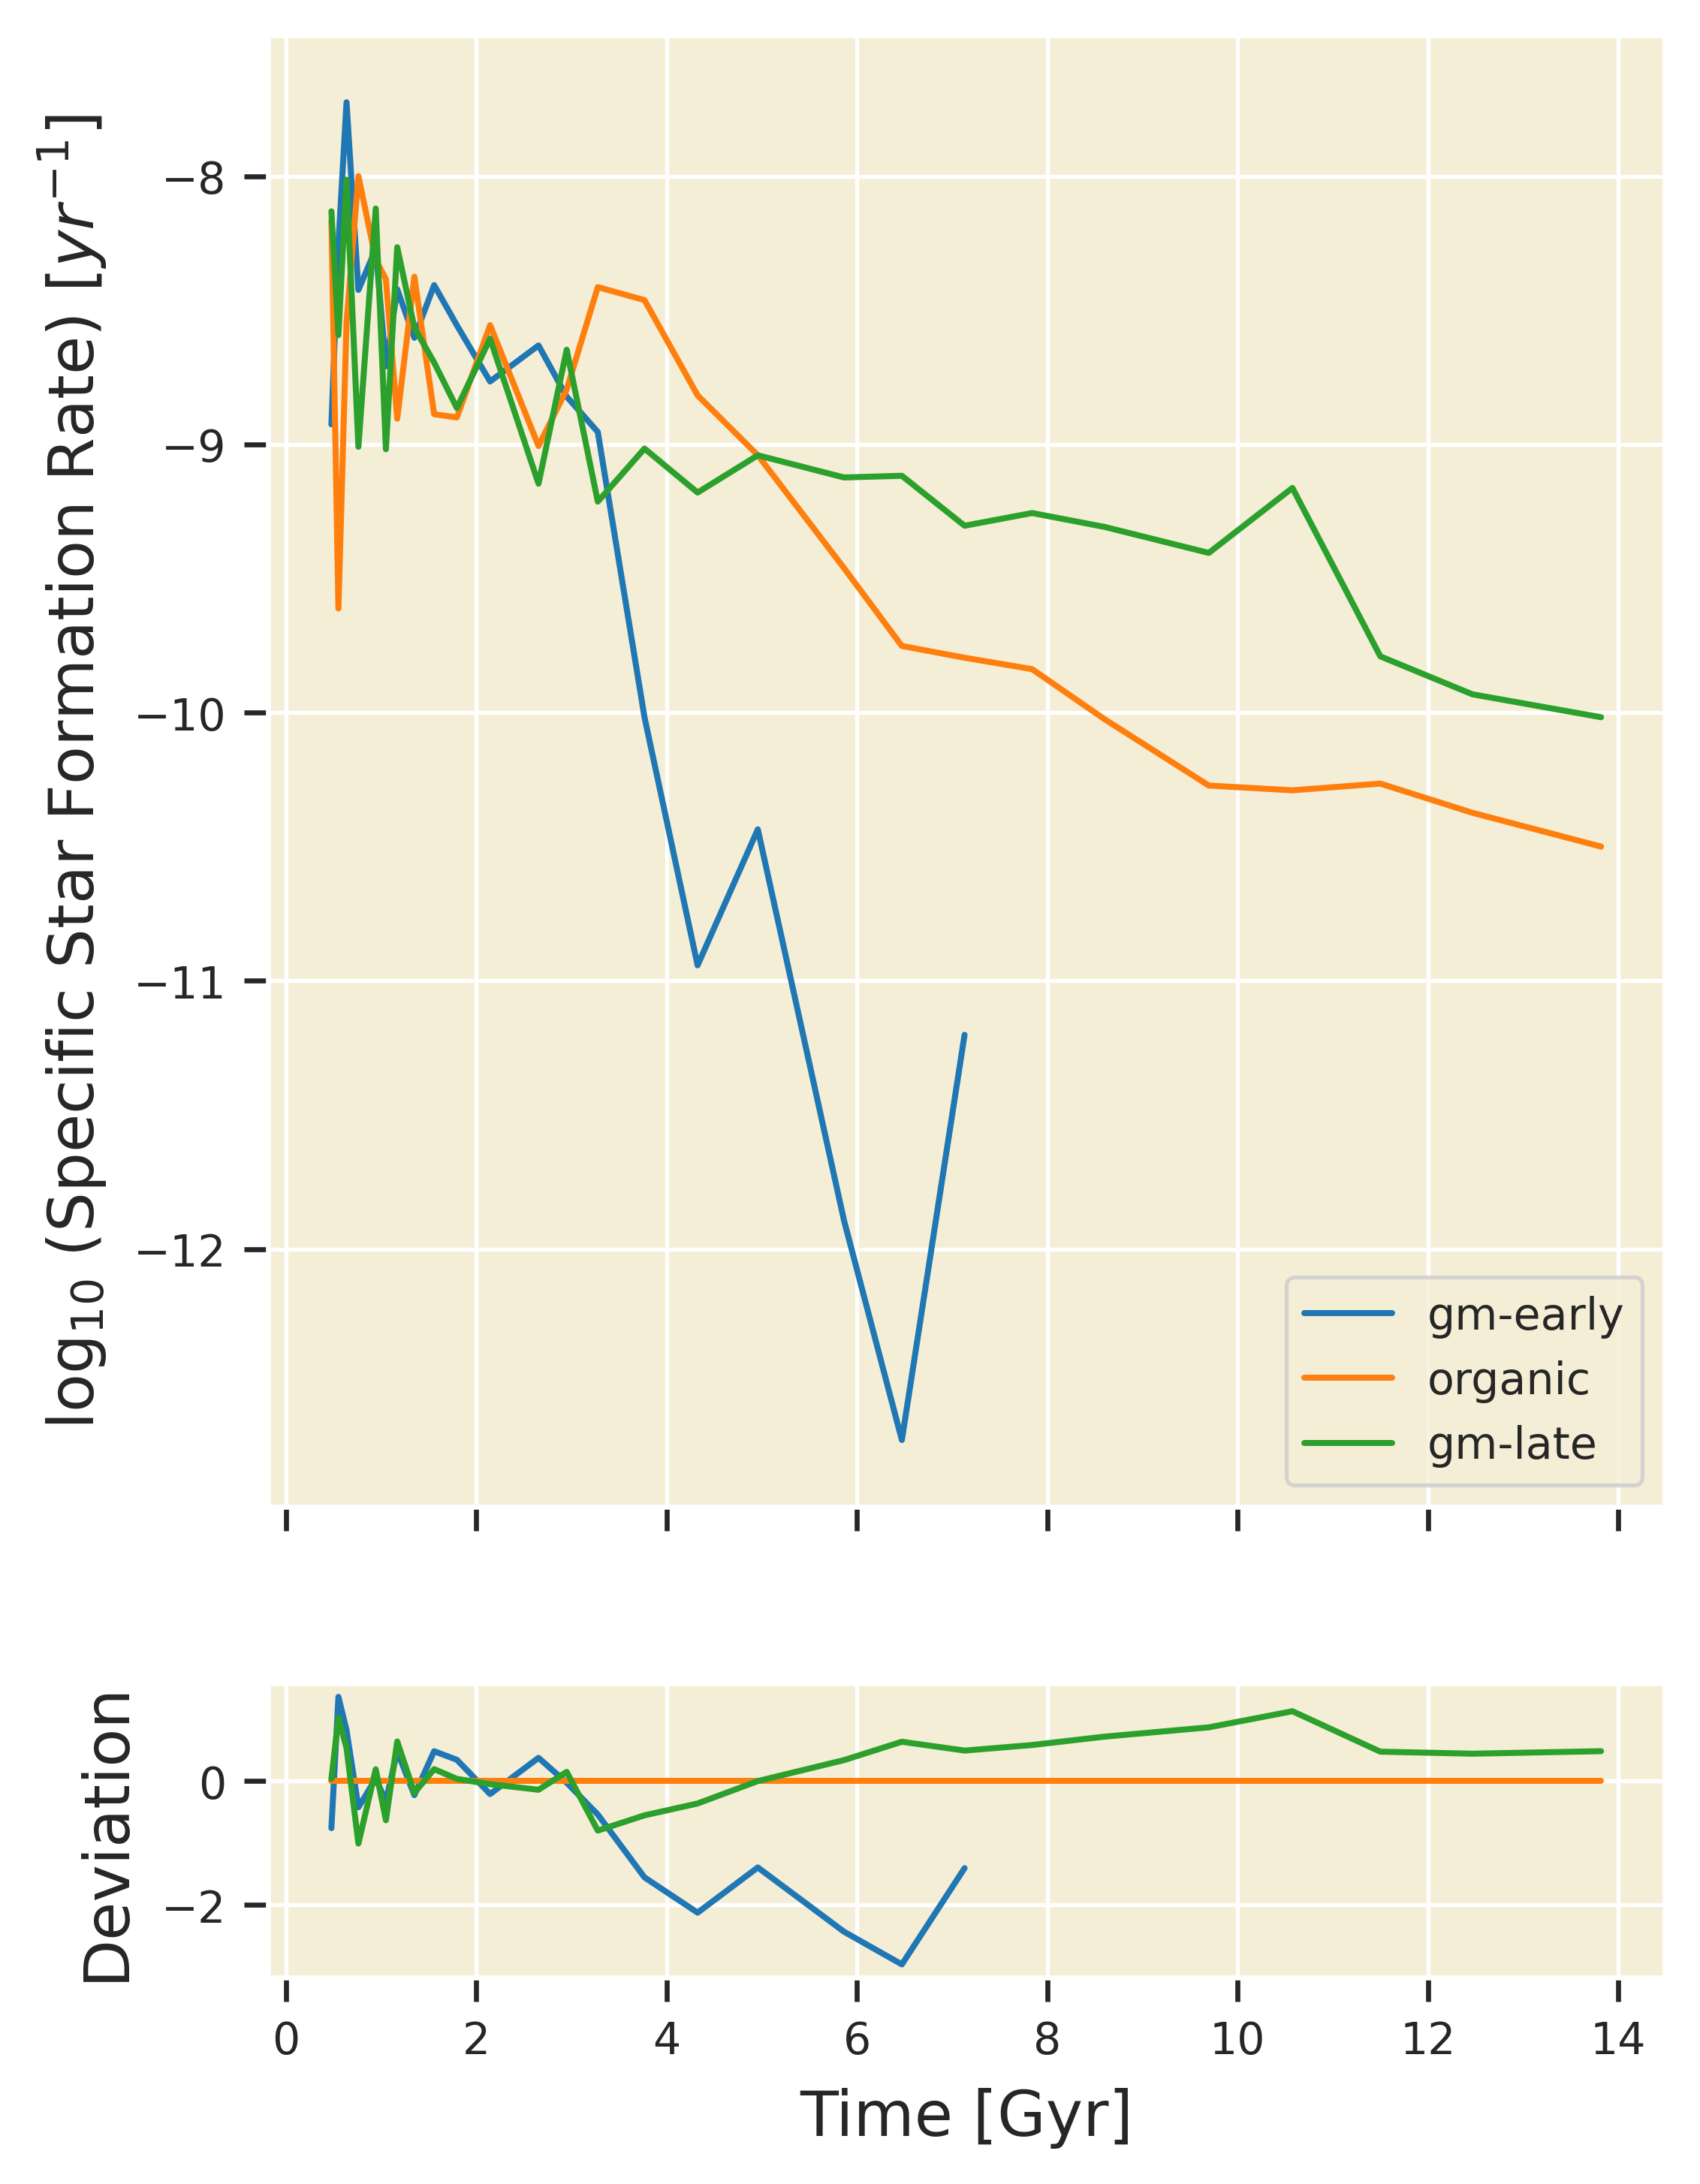
\includegraphics[width=\columnwidth]{./sSFR.png}
			\caption{Specific star formation rate variation.}
	\end{figure}

\end{document}